\section{Experiment}

\subsection{Data}
To experiment our algoritm we use the dataset 20NewsGroup \cite{Newsgroups20}.
The 20 Newsgroups data set is a collection of approximately 20,000 newsgroup 
documents, partitioned evenly across 20 different newsgroups. We use also the 
RCV1 dataset \cite{Lewis:2004:RNB:1005332.1005345}. The RCV1 dataset is a 
collection of over 800,000 text documents\\
Each document are represented by a vector using frequency-inverse document 
frequency (TFIDF) representation~\cite{doi:10.1108/eb026526}.
The term frequency-inverse document frequency is a method of weghting depicting 
the significiance of each word in a document rather a corpus.
\begin{equation}
TF(t, X) = \frac{f_{t, X}}{max_{t' \in C}f_{t', X}} 
\end{equation}
\begin{equation}
IDF(t, C) = log(\frac{N}{|X \in C : t \in X|})
\end{equation}
\begin{equation}
TFIDF(t,X,C) = TF(t, X) . IDF(t, C)   
\end{equation}
\subsection{Generate Constraint}
\subsubsection{Lexical Constraints}
To generate the set of keywords $KW$ we rank each word of each 
document of each class using TFIDF~\ref{algo:gen_kw}
\begin{algorithm}
  \SetKwInOut{Input}{input}
  \SetKwInOut{Output}{output}
  \Input{Corpus C, The number of keywords per classes $P$}
  \Output{KW}
  $KW \gets \{\}$\\
  \ForEach{Class $c_i \in C$}{
    $rank_i \gets [0 ... 0]$\\
    \ForEach{Document $X \in c_i$}{
      \ForEach{Word $w \in X$}{
        $rank_{i,w} \gets rank_{i,w} + TFIDF(w,X, C)$\\
      }
    }
  }
  \ForEach{Class $c_i, c_j \in C$}{
    \If{$c_i \neq c_j$}{
      $rank_i \gets rank_i - rank_j$\\
    }
  }
  \ForEach{Class $c_i \in C$}{
    $KW \gets KW \cup \{\{w_1, w_2 ... w_P\} : \not\exists (v_1, v_2) | v_1 \not\in 
    \{w_1, w_2 ... w_P\}, v_2 \in \{w_1, w_2 ... w_P\}, rank_{i,v_1} \ge rank_{i,v_2}\}$\\
  }
  \Return{KW}
  \caption{\label{algo:gen_kw}Extract Keywords}
\end{algorithm}
\subsubsection{Background Knowledge}
We generate pairwise constraints randomly~\ref{algo:gen_pair}
\begin{algorithm}[!h]
  \SetKwInOut{Input}{input}
  \SetKwInOut{Output}{output}
  \Input{Corpus C, The set of labels L, The number of pair $N_p$}
  \Output{Must-Link Pair ML, Cannot-Link Pair CL}
  \For{i = 1 : $N_p$}{
    Choose randomly ($X_i, X_j$)\\
    \If{$L_i == L_j$}{
      Insert ($X_i, X_j$) in ML 
    }
  }
  \For{i = 1 : $N_p$}{
    Choose randomly ($X_i, X_j$)\\
    \If{$L_i != L_j$}{
      Insert ($X_i, X_j$) in CL 
    }
  }
  \Return{ML, CL}
  \caption{\label{algo:gen_pair}Extract Pair}
\end{algorithm}
\subsection{Evaluation}
\subsubsection{Baseline Algorithm}
We evaluate our algorithm with Deep $K$-Means see in section~\ref{seq:DeepClust}.
\subsubsection{Metric}
To evaluate our algorithm and compare results with reference algorithms we can
use the NMI Metric, Accuracy Metric \cite{NMI_ACC}, and Adjusted
Rand index\cite{ARI}. 
\begin{itemize}
\item The NMI Metric is defined as follows
$$NMI(S,C) = \frac{I(S,C)}{[H(S)+H(C)]/2}$$ 
with
$I(S,C) =\sum_k \sum_f\frac{|s_k \cap c_f|}{N}log\frac{N|s_k \cap c_f|}{|s_k| |c_f|}$
and
$H(S) = -\sum_k\frac{|s_k|}{N}log\frac{N|s_k|}{|s_k|}$
\item The Accuracy is the proportion of true results among the total
  number of cases examined. The Accuracy metric is defined as follows :
$$
ACC(S,C) = \frac{1}{N}\sum_k {max}_j|s_k \cap c_j|
$$
\item Let a : the number of pairs of document in C
  that are in the same cluster in the predicted partition and in the
  same cluster in the real partition, and b : the number of pairs of
  document in C that are in different clusters in predicted partition
  and in different cluster in real partition.
  The Adjusted Rand index is defined as follows :
  $$ARI = \frac{a+b}{\binom{N}{2}}$$
\end{itemize}
\subsection{Experimental Setup}
\subsubsection{Autoencoder Architecture}
We use the same architecture used in~\cite{Deap-K-Means}. The encoder is a fully-connected 
multilayer perceptron formed by 3 hidden layers (with dimensions 500, 500, 2000) 
and an embedding layer (with dimension K, the number of cluster). 
The decoder is a mirrored version of the encoder~\ref{fig:archi}.
The ReLu activation function is used on layers, except for the third
hidden layer of encoder and decoder part.  
\begin{figure}[!h]
  \centering
  \tikzset{every picture/.style={scale=1.6}}
  \fbox{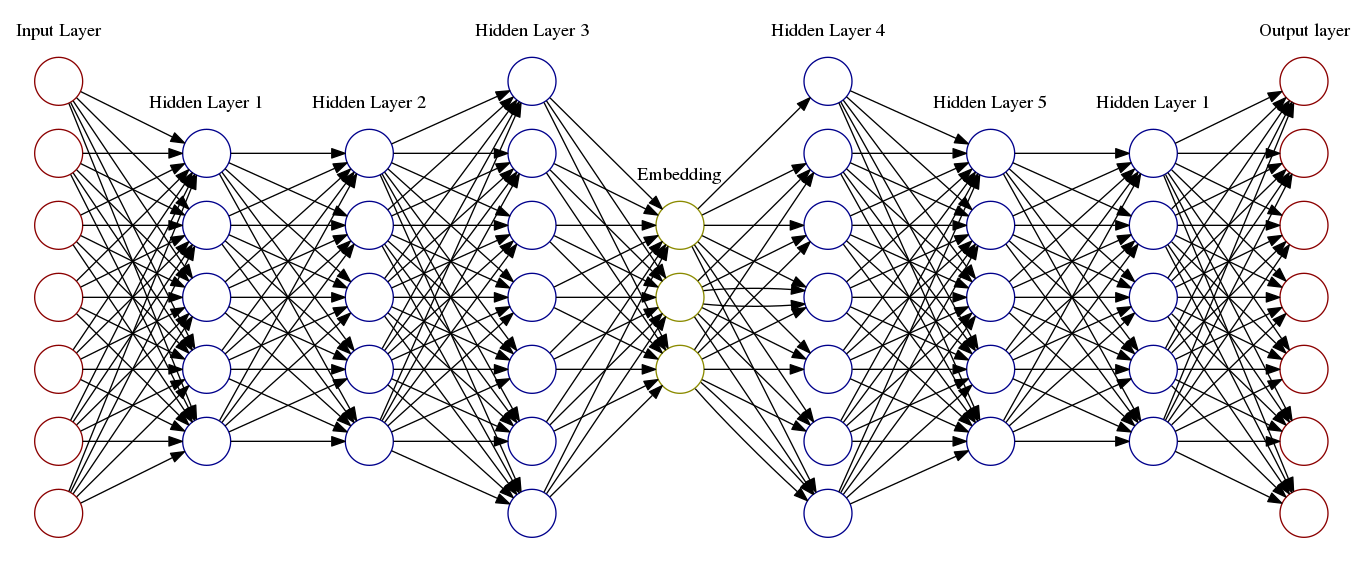
\includegraphics[scale=0.3]{parts/res/archi.png}}
  \caption{\label{fig:archi}Architecture}
\end{figure}
 
\subsubsection{Hyperparameters}
For the $\lambda$ hyerparameter we use the value defined in \cite{Deap-K-Means}. 
For the hyerparamter $\alpha_0$, we used Grid Search method for 
the hyperparameters optimization.
\begin{figure}[!h]
  \centering
  \begin{tabular}{| l | l | l | l |}
    \hline
    & 20NEWS Without noise & 20NEWS With noise & RCV1 Without noise  \\ \hline
    $\lambda$ & $10^{-1}$ & $10^{-1}$ & $10^{-1}$ \\ \hline
    $\alpha_0$ & 0 & 0 & 0 \\ \hline
    $\alpha_1$ & 0 & 0 & 0 \\ \hline
    $\alpha_2$ & 0 & 0 & 0 \\ \hline
  \end{tabular}
  \caption{\label{tab2}Hyperparameters}
\end{figure}
\subsubsection{\label{section:test1}Clustering without Noise}
The purpose of the experiment is to rediscover the different classes of the
dataset with keywords and background knowledge.

\subsubsection{\label{section:test2}Clustering with Noise}
We divide the dataset into two corpus $C_1, C_2$. Each corpus contain
ten classes. We generate keywords \ref{algo:gen_kw} and pairwise
constraints \ref{algo:gen_pair} from $C_1$. Then we add noise to the corpus
$C_1$. To add noise, we concatenate document from corpus $C_1$ with document
from corpus $C_2$.
\\The purpose of the experiment is to rediscover the different classes of the
corpus $C_1$ with keywords and background knowledge.

\subsection{Results}
In a first time, only lexical constraints have tested.
\begin{figure}[!h]
  \centering
  \begin{tabular}{| l | l | l | l | l | l | l | l | l | l | }
    \hline
    & \multicolumn{3}{|c|}{20NEWS Without noise} & \multicolumn{3}{|c|}{20NEWS With noise} & \multicolumn{3}{|c|}{RCV1 Without noise}  \\
    & ACC &ARI & NMI & ACC & ARI &NMI &ACC & ARI &NMI  \\ \hline
    Constrained Deep K-Means & 0.501& 0.353 & 0.507 & 0.404& 0.19 & 0.287 & $10^{-1}$ & $10^{4}$ & 0 \\ \hline
    Deep K-Means& 0.505 & 0.361 & 0.512 & 0.381 & 0.183 & 0.290 &   $10^{-1}$ & 0 & 0 \\ \hline
  \end{tabular}
\caption{\label{tab1}Clustering with only lexical constraints}
\end{figure}
